\section{\label{s:results}Results}

\subsection{\label{ss:meanJit}Correction of Mean Phase Jitter}

%PRL
The effect of the PFF system on the pulse-to-pulse jitter, i.e. the jitter on 
the mean phase of each beam pulse, is shown in Fig~\ref{fig:meanJit} for a 
dataset of around ten minutes duration.
The pulse-to-pulse phase jitter is reduced from  \(0.92\pm0.04^\circ\) to 
\(0.20\pm0.01^\circ\), meeting CLIC-level phase stability. 
The system acts to remove all correlation between the upstream and 
downstream phase, reducing an initial correlation of \(96\pm2\%\) to 
\(0\pm7\%\) for this dataset.
Given the incoming upstream phase jitter and 
measured upstream-downstream correlation, the performance is consistent with 
the theoretically predicted correction of \(0.26\pm0.06^\circ\).
%/PRL

Best mean jitter

\begin{figure}
 \centering
  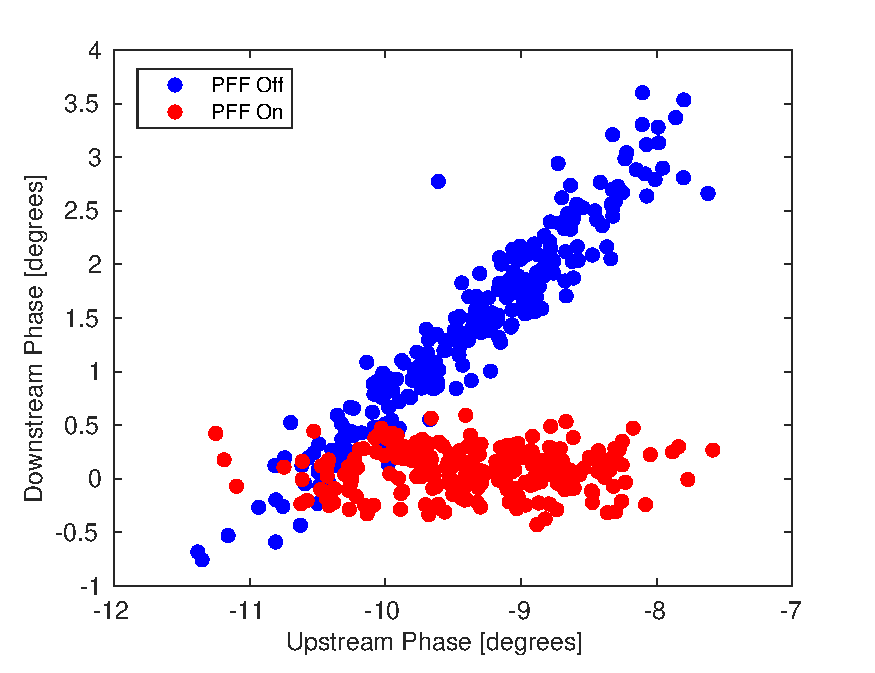
\includegraphics[width=0.6\columnwidth]{bestUpDownScatter}% Here is 
  \caption{\label{f:bestUpDownScatter}
  }
\end{figure}

\subsection{\label{ss:meanJit}Correction of Pulse Shape}
% PRL
The PFF system simultaneously corrects pulse-to-pulse phase jitter and phase 
variations within the 1.2~\(\mu s\) beam pulse at CTF3. 
Fig.~\ref{fig:shape} shows the effect of the PFF system on the intra-pulse 
phase variations. The PFF system was operated in interleaved mode, with 
the correction applied to alternating pulses only. This allows 
the initial (`PFF Off') and corrected (`PFF On') downstream phase at \(\phi_3\)
to be measured at the same time. The \(\phi_1\) (PFF input) phase 
is also shown for comparison. 

Approximately 440~ns portion of the pulse is 
within the \(\pm 6^\circ\) dynamic range of the PFF system, and can be 
corrected to zero nominal phase. 
This time duration for the full correction exceeds the CLIC drive-beam pulse 
length of 240ns and in any case the CLIC design avoids such 
a large phase sag~\cite{CLICCDR}. 
Vertical dashed lines in Fig.~\ref{fig:shape} mark the 440~ns portion of 
the pulse where full correction is possible.

Within the range the PFF system flattens the phase, and almost all variations 
are removed. 
Residual offsets are still present where there are small uncorrelated 
differences between the initial phase at \(\phi_1\) and \(\phi_3\). 
The average intra-pulse phase variation (rms) over the dataset is reduced from 
\(0.960\pm0.003^\circ\) (PFF off), to \(0.285\pm0.004^\circ\) (PFF on).
%/PRL

Best shape

\begin{figure}
 \centering
  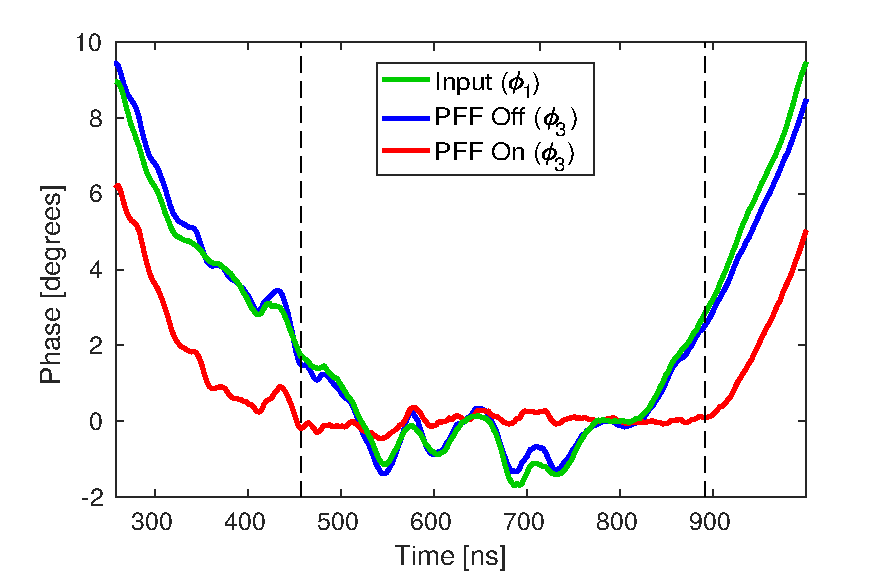
\includegraphics[width=0.6\columnwidth]{shape}% Here is 
  \caption{\label{f:shape}
  }
\end{figure}

\subsection{\label{ss:longResults}Long Term Results}

Long term correction and issues.

\begin{figure}
 \centering
  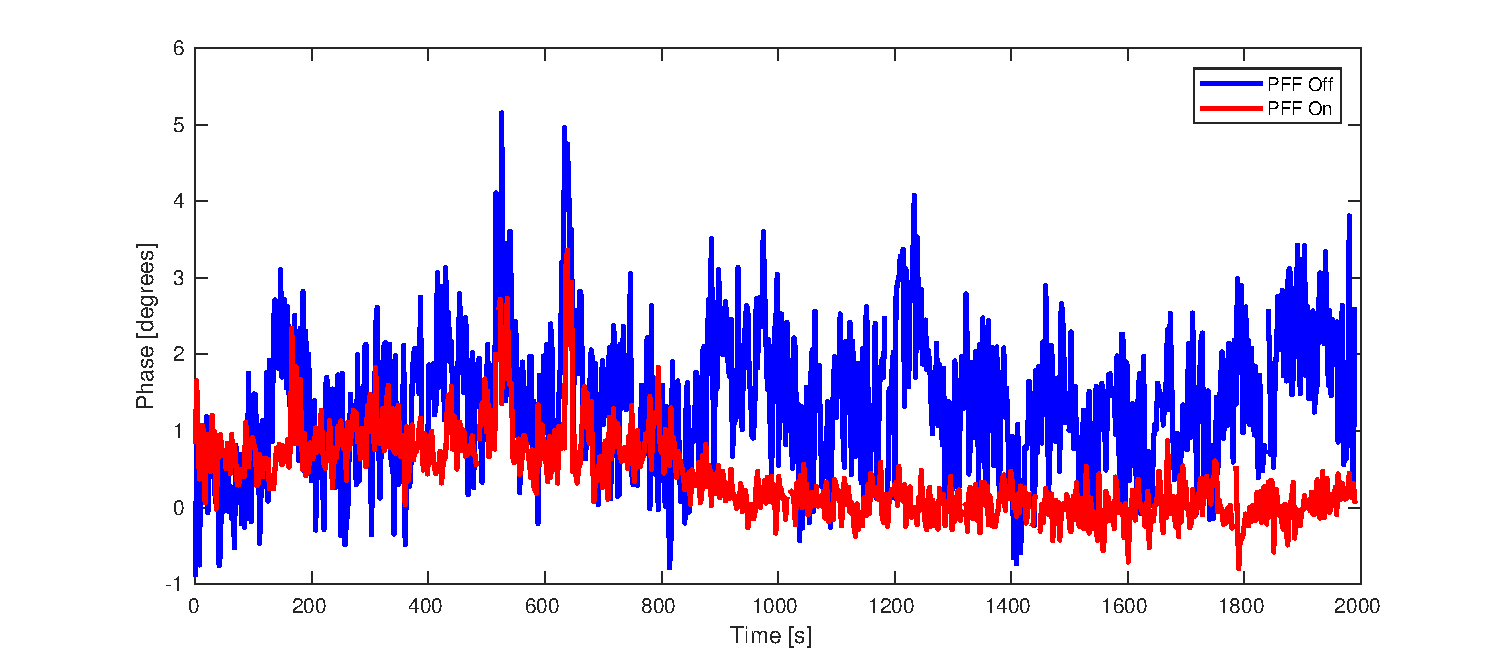
\includegraphics[width=0.6\columnwidth]{longMeanMon3}% Here is 
  \caption{\label{f:longMeanMon3}longMeanMon3
  }
\end{figure}
\begin{figure}
 \centering
  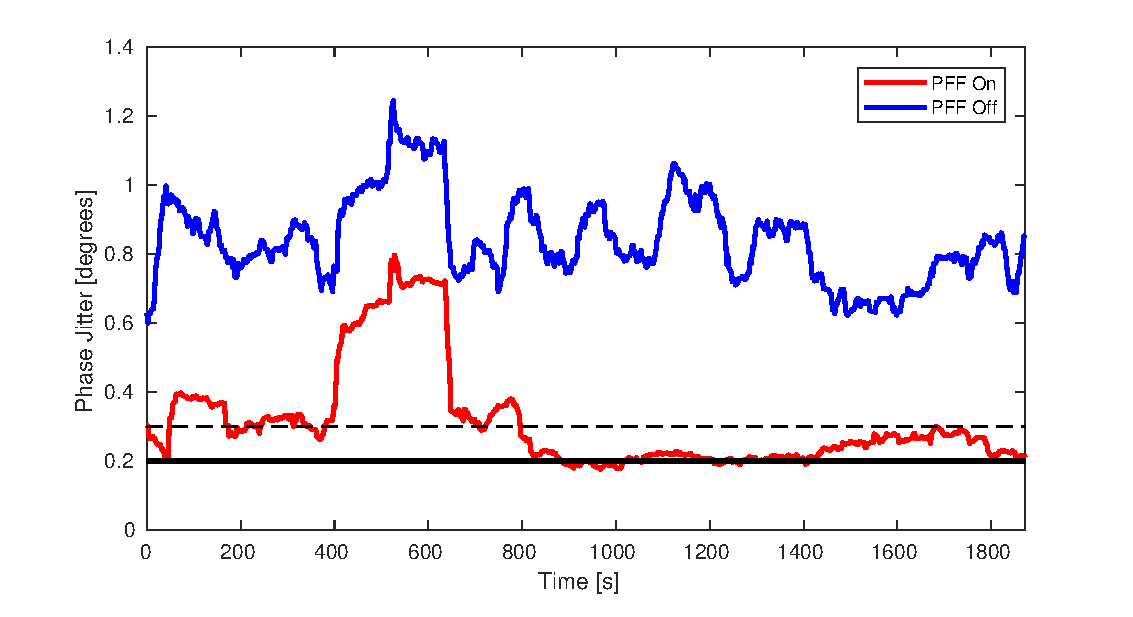
\includegraphics[width=0.6\columnwidth]{JitNext50}% Here is 
  \caption{\label{f:JitNext50}JitNext50
  }
\end{figure}
\begin{figure}
 \centering
  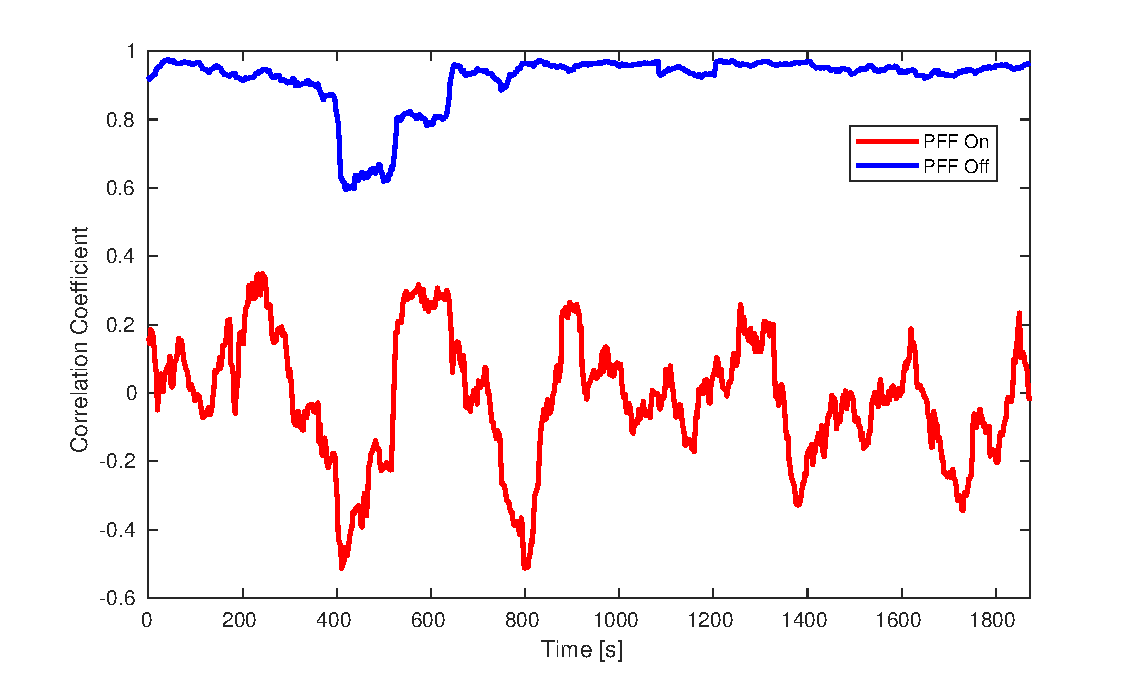
\includegraphics[width=0.6\columnwidth]{CorrNext50}% Here is 
  \caption{\label{f:CorrNext50}CorrNext50
  }
\end{figure}

